\section{Farbe von Sulfidradikalanionen}
\authors{Johannes Wörsdörfer, Jonas R. Stöckmann}

Für die blaue Farben des Stoffes Ultramarin sind die Polysulfidradikalanionen $S_3 ^{-}$ und $S_4 ^{-}$ verantwortlich (siehe Ultramarin). Um ihre Farben zu bestimmen, simulieren wir mithilfe des quantenchemischen Programmpaketes ADF \cite{ADF} das Spektrum des absorbierten Lichtes (siehe Abb. \ref{fig:3s-}). Dazu verwenden wir unrestricted TDDFT (DZ/B3LYP) und die Näherung TDA. Außerdem wird eine Kraftfeldoptimierung der Molekülgeomietrie durchgeführt. Das Ergebnis der Simulation ist, dass das $S_3^{-}$-Radikalanion bei 603 nm absorbiert. Dies wäre die Wellenlänge von orangem Licht. Der Mensch nimmt die Komplementärfarbe des absorbierten Lichtes wahr. Somit hätte der Stoff die Farbe blau. Beim $S_4^{-}$ ergibt die Simulation hingegen eine absorbierte Wellenlänge von 1025 nm (siehe Abb. \ref{fig:4s-}).
Auf Basis des Modells des Teilchens im Kasten erwarten wir, dass die Energiedifferenz sich antiproportional zum Quadrat der Länge des Kastens beziehungsweise des Moleküls $L$ verhält: $\Delta E \sim \frac{1}{L^2}$ (siehe Kapitel Teilchen im Kasten). Das heißt, je länger das Molekül ist, desto kleiner sollte die Anregungsenergie und desto größer die absorbierte Wellenlänge sein. Diese grobe Abschätzung stimmt mit unserer Simulation überein, da mit zunehmender Länge der Moleküle von $S_3^{-}$ zu $S_4^{-}$ die Anregungsenergie abnimmt.


\begin{dsafigure}
 \centering
 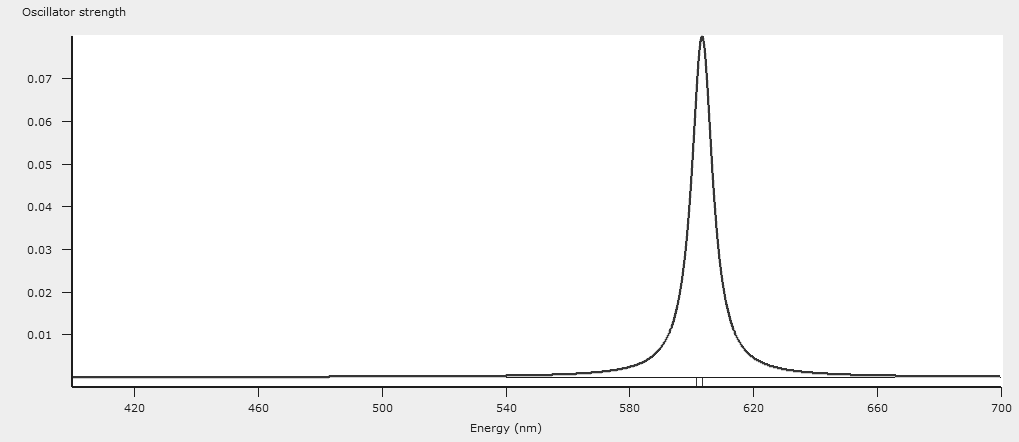
\includegraphics[width=\columnwidth]{S3-.png}
 \caption{Spektrum eines $S_3^{-}$-Radikalanions im für den Menschen sichtbaren Bereich mit einem Peak bei ca. 603 nm.}
 \label{fig:3s-}
\end{dsafigure}

\begin{dsafigure}
 \centering
 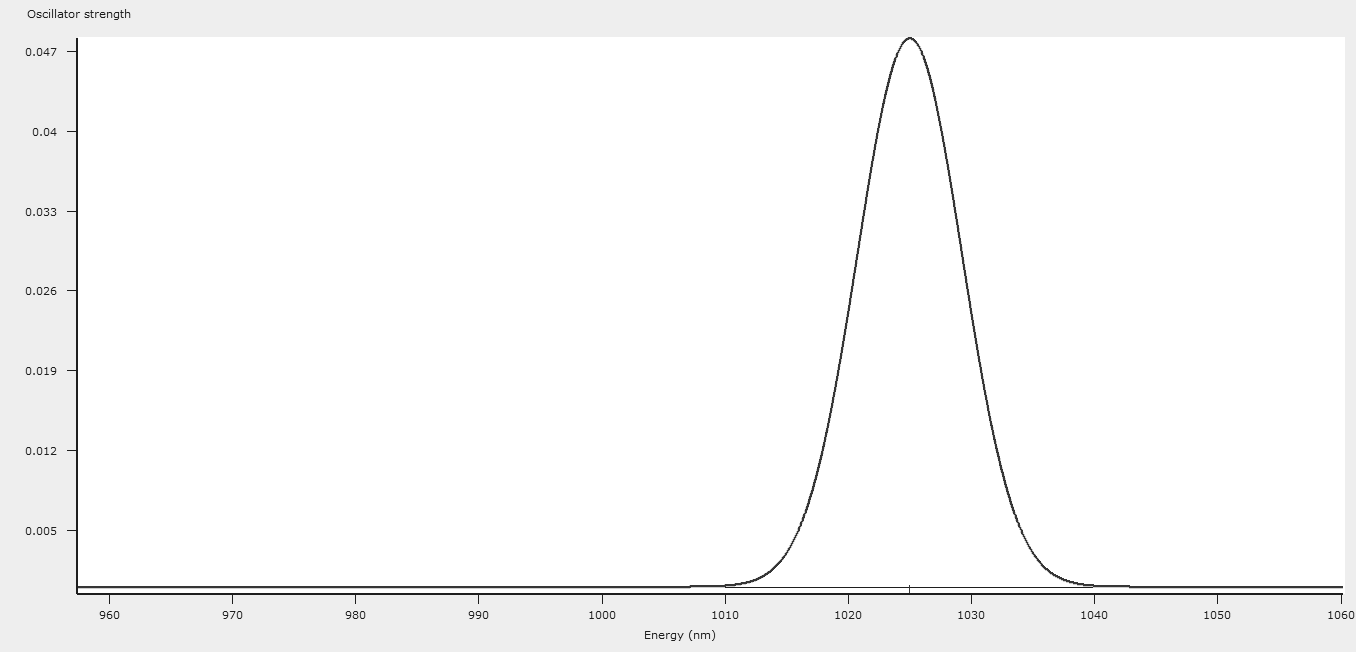
\includegraphics[width=\columnwidth]{S4-.png}
 \caption{Spektrum eines $S_4^{-}$-Radikalanions im Bereich von 960 nm bis 1060 nm mit einem Peak bei ca. 1025 nm.}
 \label{fig:4s-}
\end{dsafigure}
